\documentclass[journal,12pt,twocolumn]{IEEEtran}
\makeatletter
\@addtoreset{figure}{problem}
\makeatother
\usepackage{setspace}
\usepackage{gensymb}
\usepackage{xcolor}
\usepackage{caption}
%\usepackage{multirow}
%\usepackage{multicolumn}
%\usepackage{subcaption}
%\doublespacing
\singlespacing
\usepackage{amsmath}
\usepackage{multicol}
\usepackage{enumerate}
\usepackage{amssymb}
%\usepackage{iithtlc}
\usepackage{graphicx}
\usepackage{newfloat}
%\usepackage{syntax}
\usepackage{listings}
\usepackage{color}
\usepackage{tikz}
\usepackage[american]{circuitikz}
\usetikzlibrary{shapes,arrows}



%\usepackage{graphicx}
%\usepackage{amssymb}
%\usepackage{relsize}
%\usepackage[cmex10]{amsmath}
%\usepackage{mathtools}
%\usepackage{amsthm}
%\interdisplaylinepenalty=2500
%\savesymbol{iint}
%\usepackage{txfonts}
%\restoresymbol{TXF}{iint}
%\usepackage{wasysym}
\usepackage{amsthm}
\usepackage{mathrsfs}
\usepackage{txfonts}
\usepackage{stfloats}
\usepackage{cite}
\usepackage{cases}
\usepackage{mathtools}
\usepackage{caption}
\usepackage{enumerate}	
\usepackage{enumitem}
\usepackage{amsmath}
%\usepackage{xtab}
\usepackage{longtable}
\usepackage{multirow}
%\usepackage{algorithm}
%\usepackage{algpseudocode}
\usepackage{enumitem}
\usepackage{mathtools}

%\usepackage[framemethod=tikz]{mdframed}
\usepackage{listings}
\usepackage{listings}
    %\usepackage[latin1]{inputenc}                                 %%
    \usepackage{color}                                            %%
    \usepackage{array}                                            %%
    \usepackage{longtable}                                        %%
    \usepackage{calc}                                             %%
    \usepackage{multirow}                                         %%
    \usepackage{hhline}                                           %%
    \usepackage{ifthen}                                           %%
  %optionally (for landscape tables embedded in another document): %%
    \usepackage{lscape}     



%\usepackage{stmaryrd}


%\usepackage{wasysym}
%\newcounter{MYtempeqncnt}
\DeclareMathOperator*{\Res}{Res}
%\renewcommand{\baselinestretch}{2}
\renewcommand\thesection{\arabic{section}}
\renewcommand\thesubsection{\thesection.\arabic{subsection}}
\renewcommand\thesubsubsection{\thesubsection.\arabic{subsubsection}}

\renewcommand\thesectiondis{\arabic{section}}
\renewcommand\thesubsectiondis{\thesectiondis.\arabic{subsection}}
\renewcommand\thesubsubsectiondis{\thesubsectiondis.\arabic{subsubsection}}

% correct bad hyphenation here
\hyphenation{op-tical net-works semi-conduc-tor}

%\lstset{
%language=C,
%frame=single, 
%breaklines=true
%}

%\lstset{
	%%basicstyle=\small\ttfamily\bfseries,
	%%numberstyle=\small\ttfamily,
	%language=Octave,
	%backgroundcolor=\color{white},
	%%frame=single,
	%%keywordstyle=\bfseries,
	%%breaklines=true,
	%%showstringspaces=false,
	%%xleftmargin=-10mm,
	%%aboveskip=-1mm,
	%%belowskip=0mm
%}

%\surroundwithmdframed[width=\columnwidth]{lstlisting}
\def\inputGnumericTable{}                                 %%
\lstset{
language=C,
frame=single, 
breaklines=true
}
 

\begin{document}
%
\tikzstyle{block} = [rectangle, draw,
    text width=2em, text centered, minimum height=3em]
\tikzstyle{sum} = [draw, circle, node distance=3cm]
\tikzstyle{input} = [coordinate]
\tikzstyle{output} = [coordinate]
\tikzstyle{pinstyle} = [pin edge={to-,thin,black}]

\theoremstyle{definition}
\newtheorem{theorem}{Theorem}[section]
\newtheorem{problem}{Problem}
\newtheorem{proposition}{Proposition}[section]
\newtheorem{lemma}{Lemma}[section]
\newtheorem{corollary}[theorem]{Corollary}
\newtheorem{example}{Example}[section]
\newtheorem{definition}{Definition}[section]
%\newtheorem{algorithm}{Algorithm}[section]
%\newtheorem{cor}{Corollary}
\newcommand{\BEQA}{\begin{eqnarray}}
\newcommand{\EEQA}{\end{eqnarray}}
\newcommand{\define}{\stackrel{\triangle}{=}}

\bibliographystyle{IEEEtran}
%\bibliographystyle{ieeetr}

\providecommand{\nCr}[2]{\,^{#1}C_{#2}} % nCr
\providecommand{\nPr}[2]{\,^{#1}P_{#2}} % nPr
\providecommand{\mbf}{\mathbf}
\providecommand{\pr}[1]{\ensuremath{\Pr\left(#1\right)}}
\providecommand{\qfunc}[1]{\ensuremath{Q\left(#1\right)}}
\providecommand{\sbrak}[1]{\ensuremath{{}\left[#1\right]}}
\providecommand{\lsbrak}[1]{\ensuremath{{}\left[#1\right.}}
\providecommand{\rsbrak}[1]{\ensuremath{{}\left.#1\right]}}
\providecommand{\brak}[1]{\ensuremath{\left(#1\right)}}
\providecommand{\lbrak}[1]{\ensuremath{\left(#1\right.}}
\providecommand{\rbrak}[1]{\ensuremath{\left.#1\right)}}
\providecommand{\cbrak}[1]{\ensuremath{\left\{#1\right\}}}
\providecommand{\lcbrak}[1]{\ensuremath{\left\{#1\right.}}
\providecommand{\rcbrak}[1]{\ensuremath{\left.#1\right\}}}
\theoremstyle{remark}
\newtheorem{rem}{Remark}
\newcommand{\sgn}{\mathop{\mathrm{sgn}}}
\providecommand{\abs}[1]{\left\vert#1\right\vert}
\providecommand{\res}[1]{\Res\displaylimits_{#1}} 
\providecommand{\norm}[1]{\lVert#1\rVert}
\providecommand{\mtx}[1]{\mathbf{#1}}
\providecommand{\mean}[1]{E\left[ #1 \right]}
\providecommand{\fourier}{\overset{\mathcal{F}}{ \rightleftharpoons}}
%\providecommand{\hilbert}{\overset{\mathcal{H}}{ \rightleftharpoons}}
\providecommand{\system}{\overset{\mathcal{H}}{ \longleftrightarrow}}
	%\newcommand{\solution}[2]{\textbf{Solution:}{#1}}
\newcommand{\solution}{\noindent \textbf{Solution: }}
\providecommand{\dec}[2]{\ensuremath{\overset{#1}{\underset{#2}{\gtrless}}}}
\DeclarePairedDelimiter{\ceil}{\lceil}{\rceil}
%\numberwithin{equation}{subsection}
\numberwithin{equation}{problem}
%\numberwithin{problem}{subsection}
%\numberwithin{definition}{subsection}
\makeatletter
\@addtoreset{figure}{problem}
\makeatother

\let\StandardTheFigure\thefigure
%\renewcommand{\thefigure}{\theproblem.\arabic{figure}}
\renewcommand{\thefigure}{\theproblem}


%\numberwithin{figure}{subsection}

%\numberwithin{equation}{subsection}
%\numberwithin{equation}{section}
\numberwithin{equation}{problem}
%\numberwithin{problem}{subsection}
\numberwithin{problem}{section}
%%\numberwithin{definition}{subsection}
%\makeatletter
%\@addtoreset{figure}{problem}
%\makeatother
\makeatletter
\@addtoreset{table}{problem}
\makeatother

\let\StandardTheFigure\thefigure
\let\StandardTheTable\thetable
%%\renewcommand{\thefigure}{\theproblem.\arabic{figure}}
%\renewcommand{\thefigure}{\theproblem}

%%\numberwithin{figure}{section}

%%\numberwithin{figure}{subsection}



\def\putbox#1#2#3{\makebox[0in][l]{\makebox[#1][l]{}\raisebox{\baselineskip}[0in][0in]{\raisebox{#2}[0in][0in]{#3}}}}
     \def\rightbox#1{\makebox[0in][r]{#1}}
     \def\centbox#1{\makebox[0in]{#1}}
     \def\topbox#1{\raisebox{-\baselineskip}[0in][0in]{#1}}
     \def\midbox#1{\raisebox{-0.5\baselineskip}[0in][0in]{#1}}

\vspace{3cm}

\title{ 
	{
Stereo Speaker
	}
}

\author{Raktim Gautam Goswami and Abhishek Bairagi% <-this % stops a space
	
	
}	

\maketitle

\tableofcontents
\bigskip

\begin{abstract}
	
	In this manual we will be making a stereo speaker which will take input from a device and then amplify it and give output through speaker.
	
\end{abstract}

%\section{AC-DC Converter}
\section{Components}
\begin{table}[!h]
\centering
%%%%%%%%%%%%%%%%%%%%%%%%%%%%%%%%%%%%%%%%%%%%%%%%%%%%%%%%%%%%%%%%%%%%%%
%%                                                                  %%
%%  This is the header of a LaTeX2e file exported from Gnumeric.    %%
%%                                                                  %%
%%  This file can be compiled as it stands or included in another   %%
%%  LaTeX document. The table is based on the longtable package so  %%
%%  the longtable options (headers, footers...) can be set in the   %%
%%  preamble section below (see PRAMBLE).                           %%
%%                                                                  %%
%%  To include the file in another, the following two lines must be %%
%%  in the including file:                                          %%
%%        \def\inputGnumericTable{}                                 %%
%%  at the beginning of the file and:                               %%
%%        \input{name-of-this-file.tex}                             %%
%%  where the table is to be placed. Note also that the including   %%
%%  file must use the following packages for the table to be        %%
%%  rendered correctly:                                             %%
%%    \usepackage[latin1]{inputenc}                                 %%
%%    \usepackage{color}                                            %%
%%    \usepackage{array}                                            %%
%%    \usepackage{longtable}                                        %%
%%    \usepackage{calc}                                             %%
%%    \usepackage{multirow}                                         %%
%%    \usepackage{hhline}                                           %%
%%    \usepackage{ifthen}                                           %%
%%  optionally (for landscape tables embedded in another document): %%
%%    \usepackage{lscape}                                           %%
%%                                                                  %%
%%%%%%%%%%%%%%%%%%%%%%%%%%%%%%%%%%%%%%%%%%%%%%%%%%%%%%%%%%%%%%%%%%%%%%



%%  This section checks if we are begin input into another file or  %%
%%  the file will be compiled alone. First use a macro taken from   %%
%%  the TeXbook ex 7.7 (suggestion of Han-Wen Nienhuys).            %%
\def\ifundefined#1{\expandafter\ifx\csname#1\endcsname\relax}


%%  Check for the \def token for inputed files. If it is not        %%
%%  defined, the file will be processed as a standalone and the     %%
%%  preamble will be used.                                          %%
\ifundefined{inputGnumericTable}

%%  We must be able to close or not the document at the end.        %%
	\def\gnumericTableEnd{\end{document}}


%%%%%%%%%%%%%%%%%%%%%%%%%%%%%%%%%%%%%%%%%%%%%%%%%%%%%%%%%%%%%%%%%%%%%%
%%                                                                  %%
%%  This is the PREAMBLE. Change these values to get the right      %%
%%  paper size and other niceties.                                  %%
%%                                                                  %%
%%%%%%%%%%%%%%%%%%%%%%%%%%%%%%%%%%%%%%%%%%%%%%%%%%%%%%%%%%%%%%%%%%%%%%

	\documentclass[12pt%
			  %,landscape%
                    ]{report}
       \usepackage[latin1]{inputenc}
       \usepackage{fullpage}
       \usepackage{color}
       \usepackage{array}
       \usepackage{longtable}
       \usepackage{calc}
       \usepackage{multirow}
       \usepackage{hhline}
       \usepackage{ifthen}

	\begin{document}


%%  End of the preamble for the standalone. The next section is for %%
%%  documents which are included into other LaTeX2e files.          %%
\else

%%  We are not a stand alone document. For a regular table, we will %%
%%  have no preamble and only define the closing to mean nothing.   %%
    \def\gnumericTableEnd{}

%%  If we want landscape mode in an embedded document, comment out  %%
%%  the line above and uncomment the two below. The table will      %%
%%  begin on a new page and run in landscape mode.                  %%
%       \def\gnumericTableEnd{\end{landscape}}
%       \begin{landscape}


%%  End of the else clause for this file being \input.              %%
\fi

%%%%%%%%%%%%%%%%%%%%%%%%%%%%%%%%%%%%%%%%%%%%%%%%%%%%%%%%%%%%%%%%%%%%%%
%%                                                                  %%
%%  The rest is the gnumeric table, except for the closing          %%
%%  statement. Changes below will alter the table's appearance.     %%
%%                                                                  %%
%%%%%%%%%%%%%%%%%%%%%%%%%%%%%%%%%%%%%%%%%%%%%%%%%%%%%%%%%%%%%%%%%%%%%%

\providecommand{\gnumericmathit}[1]{#1} 
%%  Uncomment the next line if you would like your numbers to be in %%
%%  italics if they are italizised in the gnumeric table.           %%
%\renewcommand{\gnumericmathit}[1]{\mathit{#1}}
\providecommand{\gnumericPB}[1]%
{\let\gnumericTemp=\\#1\let\\=\gnumericTemp\hspace{0pt}}
 \ifundefined{gnumericTableWidthDefined}
        \newlength{\gnumericTableWidth}
        \newlength{\gnumericTableWidthComplete}
        \newlength{\gnumericMultiRowLength}
        \global\def\gnumericTableWidthDefined{}
 \fi
%% The following setting protects this code from babel shorthands.  %%
 \ifthenelse{\isundefined{\languageshorthands}}{}{\languageshorthands{english}}
%%  The default table format retains the relative column widths of  %%
%%  gnumeric. They can easily be changed to c, r or l. In that case %%
%%  you may want to comment out the next line and uncomment the one %%
%%  thereafter                                                      %%
\providecommand\gnumbox{\makebox[0pt]}
%%\providecommand\gnumbox[1][]{\makebox}

%% to adjust positions in multirow situations                       %%
\setlength{\bigstrutjot}{\jot}
\setlength{\extrarowheight}{\doublerulesep}

%%  The \setlongtables command keeps column widths the same across  %%
%%  pages. Simply comment out next line for varying column widths.  %%
\setlongtables

\setlength\gnumericTableWidth{%
	79pt+%
	100pt+%
	55pt+%
0pt}
\def\gumericNumCols{3}
\setlength\gnumericTableWidthComplete{\gnumericTableWidth+%
         \tabcolsep*\gumericNumCols*2+\arrayrulewidth*\gumericNumCols}
\ifthenelse{\lengthtest{\gnumericTableWidthComplete > \linewidth}}%
         {\def\gnumericScale{\ratio{\linewidth-%
                        \tabcolsep*\gumericNumCols*2-%
                        \arrayrulewidth*\gumericNumCols}%
{\gnumericTableWidth}}}%
{\def\gnumericScale{1}}

%%%%%%%%%%%%%%%%%%%%%%%%%%%%%%%%%%%%%%%%%%%%%%%%%%%%%%%%%%%%%%%%%%%%%%
%%                                                                  %%
%% The following are the widths of the various columns. We are      %%
%% defining them here because then they are easier to change.       %%
%% Depending on the cell formats we may use them more than once.    %%
%%                                                                  %%
%%%%%%%%%%%%%%%%%%%%%%%%%%%%%%%%%%%%%%%%%%%%%%%%%%%%%%%%%%%%%%%%%%%%%%

\ifthenelse{\isundefined{\gnumericColA}}{\newlength{\gnumericColA}}{}\settowidth{\gnumericColA}{\begin{tabular}{@{}p{79pt*\gnumericScale}@{}}x\end{tabular}}
\ifthenelse{\isundefined{\gnumericColB}}{\newlength{\gnumericColB}}{}\settowidth{\gnumericColB}{\begin{tabular}{@{}p{100pt*\gnumericScale}@{}}x\end{tabular}}
\ifthenelse{\isundefined{\gnumericColC}}{\newlength{\gnumericColC}}{}\settowidth{\gnumericColC}{\begin{tabular}{@{}p{55pt*\gnumericScale}@{}}x\end{tabular}}

\begin{tabular}[c]{%
	b{\gnumericColA}%
	b{\gnumericColB}%
	b{\gnumericColC}%
	}

%%%%%%%%%%%%%%%%%%%%%%%%%%%%%%%%%%%%%%%%%%%%%%%%%%%%%%%%%%%%%%%%%%%%%%
%%  The longtable options. (Caption, headers... see Goosens, p.124) %%
%	\caption{The Table Caption.}             \\	%
% \hline	% Across the top of the table.
%%  The rest of these options are table rows which are placed on    %%
%%  the first, last or every page. Use \multicolumn if you want.    %%

%%  Header for the first page.                                      %%
%	\multicolumn{3}{c}{The First Header} \\ \hline 
%	\multicolumn{1}{c}{colTag}	%Column 1
%	&\multicolumn{1}{c}{colTag}	%Column 2
%	&\multicolumn{1}{c}{colTag}	\\ \hline %Last column
%	\endfirsthead

%%  The running header definition.                                  %%
%	\hline
%	\multicolumn{3}{l}{\ldots\small\slshape continued} \\ \hline
%	\multicolumn{1}{c}{colTag}	%Column 1
%	&\multicolumn{1}{c}{colTag}	%Column 2
%	&\multicolumn{1}{c}{colTag}	\\ \hline %Last column
%	\endhead

%%  The running footer definition.                                  %%
%	\hline
%	\multicolumn{3}{r}{\small\slshape continued\ldots} \\
%	\endfoot

%%  The ending footer definition.                                   %%
%	\multicolumn{3}{c}{That's all folks} \\ \hline 
%	\endlastfoot
%%%%%%%%%%%%%%%%%%%%%%%%%%%%%%%%%%%%%%%%%%%%%%%%%%%%%%%%%%%%%%%%%%%%%%

\hhline{|-|-|-}
	 \multicolumn{1}{|p{\gnumericColA}|}%
	{\gnumericPB{\raggedright}\textbf{Component}}
	&\multicolumn{1}{p{\gnumericColB}|}%
	{\gnumericPB{\raggedright}\textbf{Value}}
	&\multicolumn{1}{p{\gnumericColC}|}%
	{\gnumericPB{\centering}\textbf{Quantity}}
\\
\hhline{|---|}
	 \multicolumn{1}{|p{\gnumericColA}|}%
	{\gnumericPB{\raggedright}Step Down Transformer}
	&\multicolumn{1}{p{\gnumericColB}|}%
	{\gnumericPB{\raggedright}230V AC - 12V AC - 750 mA}
	&\multicolumn{1}{p{\gnumericColC}|}%
	{\gnumericPB{\centering}1}
\\
\hhline{|---|}
	 \multicolumn{1}{|p{\gnumericColA}|}%
	{\gnumericPB{\raggedright}Diode}
	&\multicolumn{1}{p{\gnumericColB}|}%
	{}
	&\multicolumn{1}{p{\gnumericColC}|}%
	{\gnumericPB{\centering}4}
\\
\hhline{|---|}
	 \multicolumn{1}{|p{\gnumericColA}|}%
	{\gnumericPB{\raggedright}Capacitor}
	&\multicolumn{1}{p{\gnumericColB}|}%
	{\gnumericPB{\raggedright}1000 $\mu$F}
	&\multicolumn{1}{p{\gnumericColC}|}%
	{\gnumericPB{\centering}1}
\\
\hhline{|---|}
	 \multicolumn{1}{|p{\gnumericColA}|}%
	{\gnumericPB{\raggedright}Capacitor}
	&\multicolumn{1}{p{\gnumericColB}|}%
	{\gnumericPB{\raggedright}220 $\mu$F}
	&\multicolumn{1}{p{\gnumericColC}|}%
	{\gnumericPB{\centering}4}
\\
\hhline{|---|}
	 \multicolumn{1}{|p{\gnumericColA}|}%
	{\gnumericPB{\raggedright}Voltage Regulator}
	&\multicolumn{1}{p{\gnumericColB}|}%
	{\gnumericPB{\raggedright}LM7809}
	&\multicolumn{1}{p{\gnumericColC}|}%
	{\gnumericPB{\centering}1}
\\
\hhline{|---|}
	 \multicolumn{1}{|p{\gnumericColA}|}%
	{\gnumericPB{\raggedright}Jumper Wires}
	&\multicolumn{1}{p{\gnumericColB}|}%
	{\gnumericPB{\raggedright}M-M}
	&\multicolumn{1}{p{\gnumericColC}|}%
	{\gnumericPB{\centering}20}
\\
\hhline{|---|}
	 \multicolumn{1}{|p{\gnumericColA}|}%
	{\gnumericPB{\raggedright}Audio Amplifier ICs}
	&\multicolumn{1}{p{\gnumericColB}|}%
	{\gnumericPB{\raggedright}LM386}
	&\multicolumn{1}{p{\gnumericColC}|}%
	{\gnumericPB{\centering}2}
\\
\hhline{|---|}
	 \multicolumn{1}{|p{\gnumericColA}|}%
	{\gnumericPB{\raggedright}Speakers}
	&\multicolumn{1}{p{\gnumericColB}|}%
	{\gnumericPB{\raggedright}}
	&\multicolumn{1}{p{\gnumericColC}|}%
	{\gnumericPB{\centering}2}
\\
\hhline{|---|}
	 \multicolumn{1}{|p{\gnumericColA}|}%
	{\gnumericPB{\raggedright}Audio Jack}
	&\multicolumn{1}{p{\gnumericColB}|}%
	{\gnumericPB{\raggedright}}
	&\multicolumn{1}{p{\gnumericColC}|}%
	{\gnumericPB{\centering}1}
\\
\hhline{|---|}
	 \multicolumn{1}{|p{\gnumericColA}|}%
	{\gnumericPB{\raggedright}Potentiometer}
	&\multicolumn{1}{p{\gnumericColB}|}%
	{\gnumericPB{\raggedright}10k OHM}
	&\multicolumn{1}{p{\gnumericColC}|}%
	{\gnumericPB{\centering}2}
\\
\hhline{|---|}
	 \multicolumn{1}{|p{\gnumericColA}|}%
	{\gnumericPB{\raggedright}PCB}
	&\multicolumn{1}{p{\gnumericColB}|}%
	{\gnumericPB{\raggedright}}
	&\multicolumn{1}{p{\gnumericColC}|}%
	{\gnumericPB{\centering}1}
\\
\hhline{|-|-|-|}
\end{tabular}

\ifthenelse{\isundefined{\languageshorthands}}{}{\languageshorthands{\languagename}}
\gnumericTableEnd

\caption{}
\label{table:components}
\end{table}
%\begin{enumerate} 
%\item Step-Down Transformer (230 V AC to 12V-0-12V , 750 mA)
%\item Diodes - 4
%\item Capacitor - 100 $\mu$ F , 0.1 $\mu$ F - 2 no's
%\item Voltage Regulator - LM7809
%\item Audio Amplifier IC - LM386
%\end{enumerate}
\section{Circuit Diagram for converting 230V AC to 12V DC }
The circuit diagram is shown in \ref{fig1}
\begin{figure}[!h]
\centering
\resizebox {\columnwidth} {!} {
       \begin{circuitikz}
      \draw (0,-0.1)
    to[sV= $ V_{s}$] (0,2) 
    %to [short] (1,3)
    %to [short] (1,2.5)
    (1,2) node [transformer core](T){}
      %(T.base) node{K}
    %(3,1.5) to [open,rotate=90,v=$12V \hspace{0.2cm} AC$] (3,-0.1) 
    %to [short] (2, -0.6] 
    (2,2) to [short] (2,2.5)
    to [short] (4,2.5)
    (2.5,1) to [D,l=$D1$] (4,2.5)
    to [D,l=$D2$] (5.5,1)
    to [D,l=$D3$] (4,-0.1)
    (2.5,1) to [D,l=$D4$] (4,-0.1)
    to [short] (4,-0.6)
    to [short] (2,-0.6)
    to [short] (2,-0.1)
    (5.5,1) to [short] (6.5,1)
    (2.5,1) to [short] (2.5,-3)
    to [short] (9,-3)
    (6,1) to [C,l=$1000 \mu F$] (6,-3)
    
    (7,1) node[block]{{\textbf{LM 7809}}}
    (7.6,1) to [short] (9,1)
    to [open, v=$9V $] (9,-3)
    to [short] (2.5,-3)
    
    
    
    %to [short] (7,3)
    %to [L=$L$,i>^=$I_L$, v=$v_{L}$] (3,3)
    %to[C=$C$,i>^=$I_C$,v=$v_{C}$] (3,0)
    %(3,3) to [short] (5,3)
    %to [R=$R_L$,i>^=$I_o$,v=$v_{o}$] (5,0)
    %to[short] (0,0)
    ;  
    \end{circuitikz}
}
\caption{AC-DC circuit diagram} 
\label{fig1}
\end{figure}

\begin{problem}
Measure the voltage and frequency at the input and output of transformer.
\end{problem}

\solution
The input voltage is 230V @ 50 Hz and output of transformer is approximately 20V @ 50 Hz.

%\begin{figure}
 %      \centering  

\section{Connections}
%\subsection{Steps to Convert 230V AC to 5V , 2A DC}
%\subsubsection{Step Down the Voltage Level}
%\begin{problem}
%How can you convert 23V AC voltage to 12V DC voltage?
%\end{problem} 
%230V AC is converted into 12V AC using a step-down transformer. 
%12V output of step-down transformer is an RMS %value and its peak value is given by the product %of square root of two with RMS value, which is %approximately 17V.
\begin{problem}
Connect the 230V AC supply to the input of the step-down transformer.
%Connect the 230V AC supply to the input of the step-down transformer.
\end{problem}
\begin{problem}
Connect the 4 diodes in bridge as shown in fig \ref{fig1} .
%Connect the 230V AC supply to the input of the step-down transformer.
\end{problem}
\begin{problem}
Connect the 12V and GND wires of the transformer to the to the juction of diodes D1, D2 and D3 , D4 .
%Connect the 230V AC supply to the input of the step-down transformer.
\end{problem}
%Connect the 230V AC supply to the input of the step-down transformer.

%\subsubsection{Convert AC to DC}
%\begin{problem}
%Connect the 4 diodes in bridge as shown in fig \ref{fig1} .
%\end{problem}
%\begin{problem}
%Connect the 12V and OV wires of the transformer to the to the juction of diodes D1, D2 and D3 , D4 .   
%\end{problem}
\begin{problem}
The observed output of the Bridge Rectifier between junctions of D1,D4 and D2,D3 on  oscilloscope is as shown in Fig. \ref{fig2}.
\end{problem}


%AC power can be converted into DC using one of the power electronic converters called as Rectifier. The bridge rectifier is frequently used for converting AC to DC. \\
%Bridge rectifier consists of four diodes which are connected in the form a bridge. We know that the diode is an uncontrolled rectifier which will conduct only forward bias and will not conduct during the reverse bias. If the diode anode voltage is greater than the cathode voltage then the diode is said to be in forward bias. During positive half cycle, diodes D2 and D4 will conduct and during negative half cycle diodes D1 and D3 will conduct. Thus, AC is converted into DC; here the obtained is not a pure DC as it consists of pulses. Hence, it is called as pulsating DC power. But voltage drop across the diodes is (2*0.7V) 1.4V; therefore, the peak voltage at the output of this retifier circuit is 15V (17-1.4) approx.

\begin{figure}[h]
\centering
	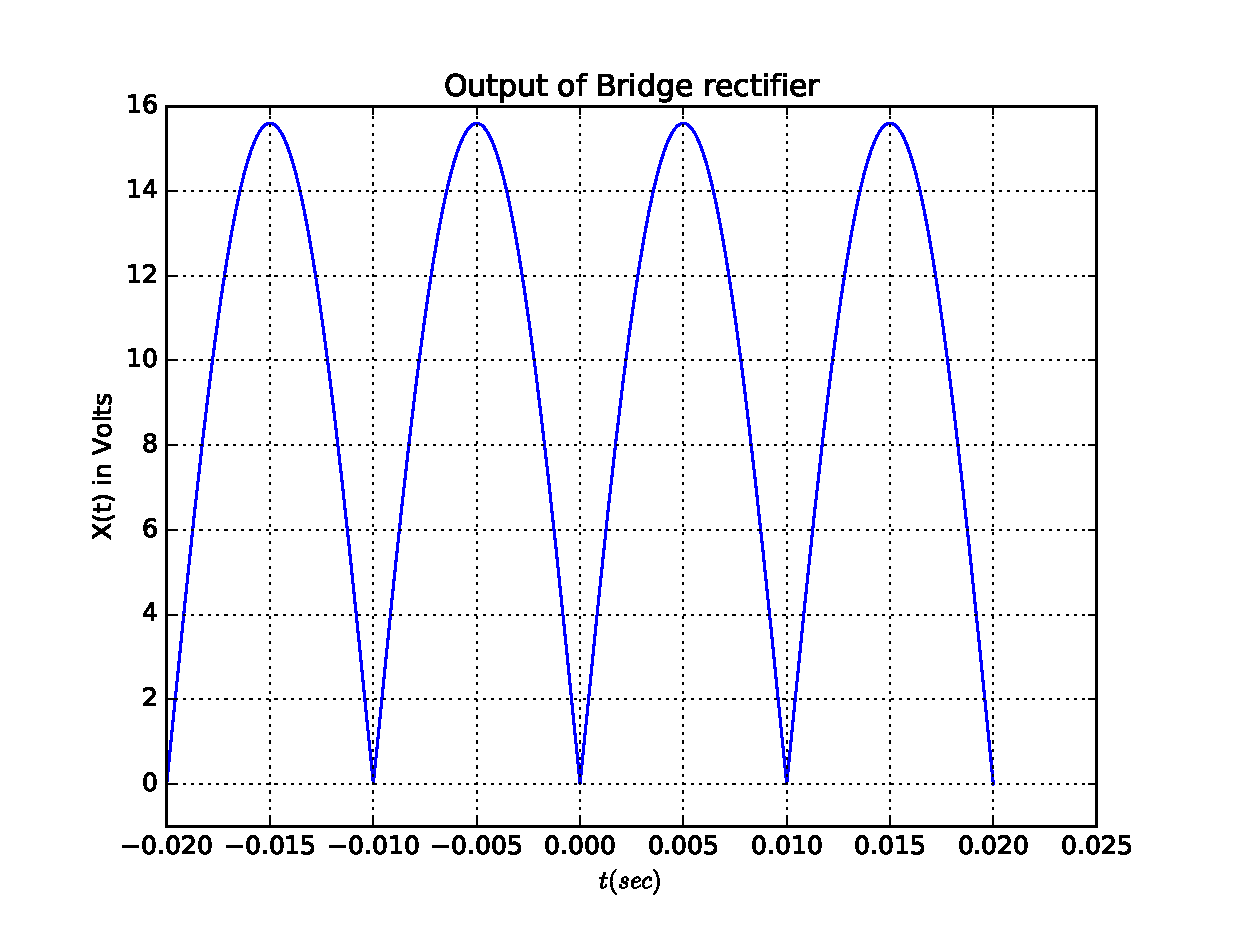
\includegraphics[scale=0.4]{./figs/sine.eps}
	\caption{Rectified Wave}  \label{fig2}
    \end{figure}

\section{Functioning}
\subsection{Ripple Filter}
%\begin{problem}
%What is the role of the capacitor in the circuit?
%\end{problem}
%\solution
%The output of the diode bridge is a DC consisting of ripples also called as pulsating DC. This pulsating DC can be filtered using an inductor filter or a capacitor filter or a resistor-capacitor-coupled filter for removing the ripples. Consider a capacitor filter which is frequently used in most cases for smoothing.
\begin{problem}
The output of the diode bridge is a DC consisting of ripples also called as pulsating DC. This pulsating DC can be filtered using  capacitor filter.Connect a capacitor across the bridge as shown in figure 2.0. 
\end{problem}
\begin{problem}
The observed output of the capacitor filter is as shown in Fig.\ref{fig3}.
\end{problem}

\begin{figure}[h]
\centering
	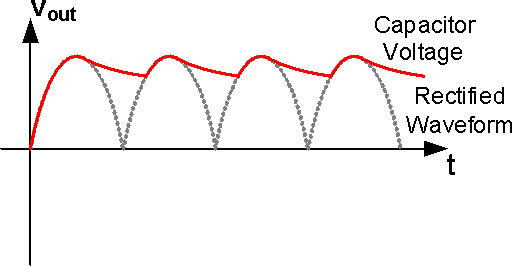
\includegraphics[scale=0.4]{./figs/cap.png}
	\caption{Rectified Wave with Capacitive filter}  \label{fig3}
    \end{figure}

\subsection{Voltage Regulator}
The pin description of LM7809 is shown in Fig. \ref{fig4}
\begin{figure}[h]
\centering
	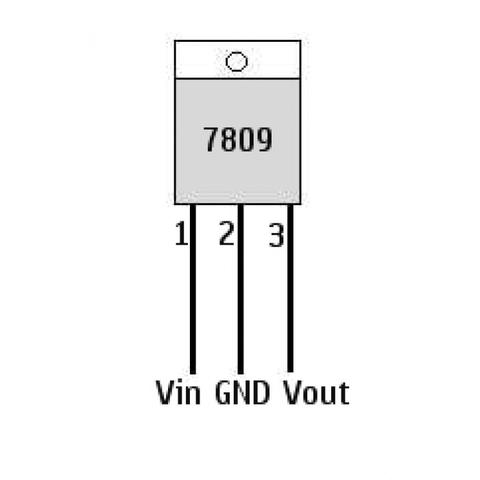
\includegraphics[scale=0.4]{./figs/ic.jpg}
	\caption{LM7809}  \label{fig4}
    \end{figure}

\begin{problem}
Connect pin 1 and pin 2 of LM7809 to positive and Ground terminals of 220 uF capacitor and pin 3 to the positive of another 220 uF capacitor. Connect other end of capacitor to ground. The circuit is as shown in Fig. \ref{lm7809} 
\begin{figure}[h]
\centering
	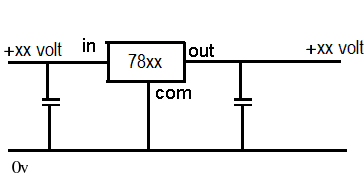
\includegraphics[scale=0.5]{./figs/lm7809.png}
	\caption{LM 7809 connections}  \label{lm7809}
    \end{figure}
\end{problem} 
\begin{problem}
Measure the Voltage across pin 3 and Ground of LM7805. What do you observe?
\end{problem}
\solution
The output voltage is observed to be 9V.

\section{Circuit for audio amplification}

%\begin{problem}
%What is the role of the capacitor in the circuit?
%\end{problem}
%\solution
%The output of the diode bridge is a DC consisting of ripples also called as pulsating DC. This pulsating DC can be filtered using an inductor filter or a capacitor filter or a resistor-capacitor-coupled filter for removing the ripples. Consider a capacitor filter which is frequently used in most cases for smoothing.
\begin{problem}
Connect the 9V obtained from the previous circuit to pin 6  and ground to pin 2 and 4 of LM386 IC.
\end{problem}
\begin{problem}
Connection points for the audio jack are as shown in Fig.\ref{fig5}
\end{problem}
\begin{figure}[h]
\centering
	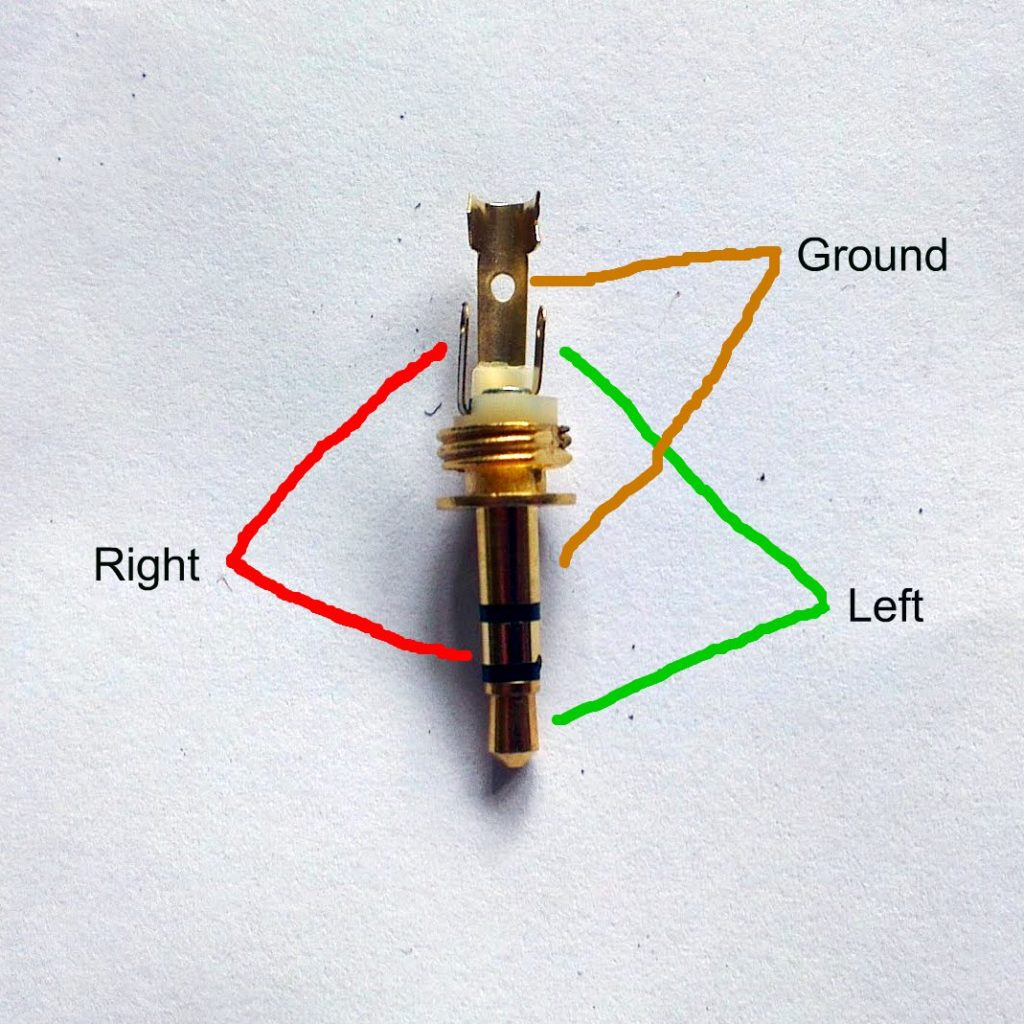
\includegraphics[scale=0.2]{./figs/jack.jpg}
	\caption{Audio Jack connection points}  \label{fig5}
    \end{figure}
\begin{problem}
Connect one input from audio jack to pin 3 of LM386 IC with a variable resistor in series (you can use potentiometer instead of variable resistor). See Fig. \ref{fig6} for reference
\end{problem}
\begin{figure}[h]
\centering
	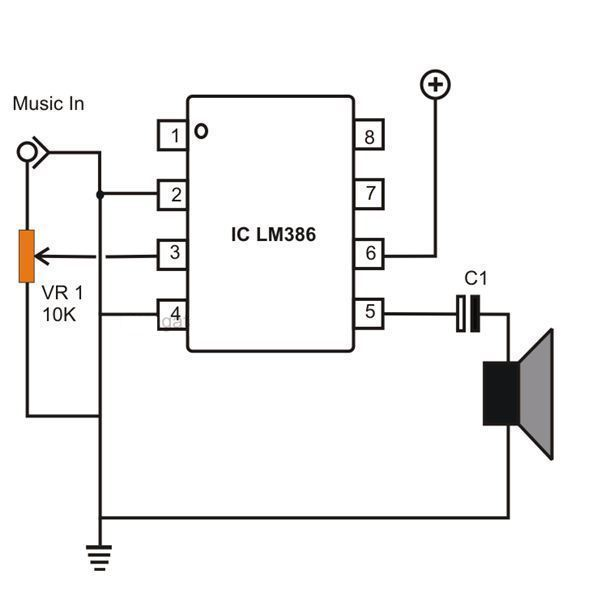
\includegraphics[scale=0.4]{./figs/LM386.jpg}
	\caption{LM386}  \label{fig6}
    \end{figure}


\begin{problem}
Connect one  wire of speaker to pin 5 of LM386 through a 220 uf (C1) capacitor and other to ground.
\end{problem}
\begin{problem}
Make the same circuit with another LM386 IC(This time use the other input of audio jack and connect remaining wire of audio jack to ground).
\end{problem}
\begin{problem}
Now connect audio jack to an input device and turn on power supply. Try changing volume by potentiometer.
\end{problem}




\end{document}
